\documentclass[12pt,a4paper,titlepage]{article}
\usepackage[utf8]{inputenc}
\usepackage[T1]{fontenc}
\usepackage[top=3cm, bottom=3cm, left=2cm, right=2cm]{geometry}
\usepackage{textcomp}
\usepackage{amsmath}
\usepackage{amsfonts}
\usepackage{amssymb}
\usepackage{amsthm}
\usepackage{titlesec}
\usepackage{fancyhdr}
\usepackage{lastpage}
\usepackage{fix-cm}
\usepackage{graphicx}
\usepackage{hyperref}
\usepackage{xcolor}
\usepackage{mdwlist}
\usepackage{listings}
\usepackage{float}
\usepackage{wrapfig}
\usepackage{datetime}
\usepackage[perpage,para,bottom,marginal]{footmisc}
\usepackage{listings}
\usepackage{caption}
\usepackage{enumitem}
\usepackage{multicol}
\usepackage[cmtip,all]{xy}
\newdateformat{dmny}{\monthname[\THEMONTH] \THEYEAR}
\newdateformat{dyo}{\THEYEAR}
\setlength{\headheight}{30pt}
\pagestyle{fancy}

\author{Nicolas Hafner}
\lhead{Nicolas Hafner}
\title{Analysis II}
\chead{Analysis II}
\rhead{Zürich, \dmny\today}
\cfoot{\thepage\ / \pageref{LastPage}}
\lfoot{\copyright \dyo\today TymoonNET/NexT}
\date{\d_mny\today}

\newcommand{\longsquiggly}{\xymatrix{{}\ar@{~>}[r]&{}}}
\renewcommand{\Re}{\operatorname{Re}}
\renewcommand{\Im}{\operatorname{Im}}
\renewcommand{\arg}{\operatorname{arg}}
\renewcommand{\d}{\partial}
\newcommand{\arsinh}{\operatorname{arsinh}}
\newcommand{\arcosh}{\operatorname{arcosh}}
\newcommand{\artanh}{\operatorname{artanh}}
\newcommand{\setC}{\mathbb{C}}
\newcommand{\setR}{\mathbb{R}}
\newcommand{\setZ}{\mathbb{Z}}
\newcommand{\setN}{\mathbb{Z}^{\geq0}}
\newcommand{\Graph}{\operatorname{Graph}}

\begin{document}	
\begin{center}{\bfseries\Huge Analysis II - 2014.03.24}\end{center}
\textit{Erinnerung}: Kritischer Punkt: $\nabla f=0$, nicht ausgeartet: $\det\nabla^2f\neq 0$, etc. See prev. doc. \\
\\
\textit{Beispiel}: Zwei Partikel an den Stellen $0<x<y<1$ mit Abstossungskräften proportional zum Kehrwert des Abstandes zum Rand und dem anderen Partikel. Wo ist ein Gleichgewicht, und ist es \emph{stabil}? \\
\\
\textit{Lösung}: Energie: $E=\log\frac{1}{x}+2\log\frac{1}{y-x}+\log\frac{1}{1-y}=-\log x-2\log(y-x)-\log(1-y)$ \\
$\nabla E=(-\frac{1}{x}+\frac{2}{y-x},\;\frac{-2}{y-x}+\frac{1}{1-x})$ \\
Krit. Punkte: $\frac{1}{x}=\frac{2}{y-x} \iff y-x=2x,\; \frac{1}{1-y}=\frac{2}{y-x}\iff y-x=2(1-y) \Rightarrow x=\frac{1}{4}\land y=\frac{3}{4}$ \\
$\nabla^2E=\begin{pmatrix}
  \frac{1}{x^2}+\frac{2}{(y-x)^2} & \frac{-2}{(y-x)^2} \\
  \frac{-2}{(y-x)^2} & \frac{2}{(y-x)^2}+\frac{1}{(1-y)^2} \\
\end{pmatrix} \Rightarrow \nabla^2E(\frac{1}{4},\frac{3}{4})=8\begin{pmatrix}3&-1\\-1&3\end{pmatrix}$ \\
$\Rightarrow \left|\begin{matrix}3-\lambda & -1 \\ -1 & 3-\lambda\end{matrix}\right|=(3-\lambda)^2-(-1)^2=\lambda^2-6\lambda+8=(\lambda-2)(\lambda-4) \Rightarrow \text{EWe}>0 \Rightarrow \text{pos.def.}$ \\
$\Rightarrow$ E hat isoliertes, lokales Minimum in $(\frac{1}{4},\;\frac{3}{4}) \Rightarrow$ stabil.

\section*{Globale Extrema}
\textit{Erinnerung}: Jede stetige Funktion $f:K\to\setR$ für $\varnothing\neq K\subset\setR^n$ kompakt hat ein Minimum und ein Maximum. \\
\\
\textit{Fakt}: Sei $f$ diff'bar. Jede Extremalstelle von $f$ ist entweder ein kritischer Punkt von $f\mid K^\circ$ (Inneres) oder eine Extremalstelle von $f\mid\d K$ (Rand). Für den Rand teilen wir $\d K$ in Stücke auf und eliminieren auf jedem eine Variable. \\
\\
\textit{Beispiel}: Finde die Extrema von $f(x,y):=x^3-18x^2+81x+12y^2-144y+24xy$ auf $B:=\{(x,y)\mid x\geq 0,y\geq 0,x+y\leq 10\}$ \\
\\
\textit{Lösung}: Auf $B^\circ: \nabla f=(3x^2-36x+81+24y,\; 24y-144+24x)$ \\
Kritische Punkte: Diff: $3x^2-36x+81+144-24x=0 \Rightarrow x^2-20x+75=0 \Rightarrow (x-5)(x-15)=0$ \\
Da $15$ sowieso nicht im Bereich liegt, müssen wir nur $5$ probieren: $24(-6+5)=0 \Rightarrow y=1$ \\
$\Rightarrow$ Kandidat $(5,1)$ \\
\\
Auf Teilmenge $y=0,\; 0<x<10,\; f(x,0)=x^3-18x^2+81x \Rightarrow \frac{\d}{\d x}(x,0)=3(x-3)(x-9)$
\begin{wrapfigure}{r}{6cm}
  \centering
  \begin{tabular}{c|c|l}
    $(x,y)$ & $f(x,y)$ & \\
    \hline
    $(5,1)$ & $68$ & \\
    $(3,0)$ & $108$ & \\
    $(9,0)$ & $0$ & \\
    $(0,6)$ & $-432$ & MIN\\
    $(5,5)$ & $260$ & MAX\\
    $(0,0)$ & $0$ & \\
    $(10,0)$ & $10$ & \\
    $(0,10)$ & $-240$ &
  \end{tabular}
\end{wrapfigure}
$\Rightarrow$ Kandidaten $(3,0)\quad(9,0)$ \\
\\
Auf Teilmenge $x=0,\; 0<y<10 $ \\
$\Rightarrow$ Kandidaten $(0,6)\quad(0,0)$ \\
\\
Auf Teilmenge $x+y=10,\; 0<y<10 $ \\
$\Rightarrow$ Kandidaten $(5,5)$ \\
\\
$\Rightarrow$ Eckpunkte $(0,10)\quad(10,0)\quad(0,0)$ \\

\section*{Implizite Funktionen}
Sei $U\subset\setR^{n+1}$ offen und $f:U\to\setR$ $k\geq 1$ mal stetig diff'bar. \\
\textit{Definition}: Ein Punkt $x\in U$ mit $\nabla f(x)\neq(0..0)$ heisst \emph{regulärer Punkt von $f$}. \\
\\
\textit{Satz}: Sei $\xi=(\xi_1..\xi_{n+1})$ ein regulärer Punkt von $f$ mit $\frac{\d f}{\d x_{n+1}}(\xi)\neq 0$ und \\
$\xi\in G:=\{x\in U\mid f(x)=0\}$. Dann existieren eine offene Teilmenge $V\times I\subset U$ mit $\xi\in V\times I$ mit $V\subset\setR^n,\; I\subset\setR$ und eine $k$-mal stetig diff'bare Funktion $\varphi:V\to I$, sodass $\Graph(\varphi)=G\cap(V\times I)$ ist. Für die gilt also $\varphi(\xi_1..\xi_n)=\xi_{n+1}$ und $\forall 1\leq i\leq n: \frac{\d\varphi}{\d x_i}(\xi_1..\xi_n)=-\frac{\d f}{\d x_i}(\xi)/\frac{\d f}{\d x_{n+1}}(\xi)$ \\
\\
\begin{figure}[h!]
  \begin{center}
    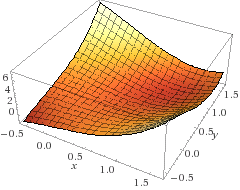
\includegraphics{WolframAlpha--x_3_y_3_3xy__3D_plot__2014_03_24_0348.png}
  \end{center}
\end{figure}
\textit{Beispiel}: $G:=\{(x,y)\in\setR^2\mid f(x,y)=0\}$ und $f(x,y):=x^3+y^3-3xy$ \\
Die maximalen Zweige von $G$, die Graph einer Funktion sind, sind $\{(x,y)\in G\mid x<0\},\quad $\\
$\{''\mid x>0\land y<0\},\quad \{''\mid 0<x<\sqrt[3]{4}\land 0<y<\sqrt{x}\},\quad \{''\mid 0<x<\sqrt[3]{4}\land y>\sqrt{x}\}$ \\
\\
$(\xi,\eta)=(\frac{2}{3},\frac{4}{3}) \Rightarrow f(\xi,\eta)=(\frac{2}{3})^3+(\frac{4}{3})^3-3\frac{2}{3}\frac{4}{3}=0 \Rightarrow (\xi,\eta)\in G$ \\
$\nabla f=(3x^2-3y,\; 3y^2-3x) \quad \nabla f(\xi,\eta)=(-\frac{8}{3},\;\frac{10}{3}) \quad \frac{d\varphi}{d x}(\xi)=-(-\frac{8}{3})^3/(\frac{10}{3})^3=\frac{4}{5}$ \\
\\
$f(x,y)=f(\xi,\eta)+\nabla f(\xi,\eta)(x-\xi,\;y-\eta)+o(|(x-\xi,\;y-\eta)|)$ \\
$\Rightarrow$ Falls $\nabla f(\xi,\eta)\neq(0,0)$ ist, ist $f(\xi,\eta)+\nabla f(\xi,\eta)(x-\xi,y-\eta)=0$ die Gleichung der Tangente an die Kurve $f(x,y)=0$ in $(\xi,\eta)$.
\end{document}